\documentclass{beamer}
\usepackage[utf8]{inputenc}
\usepackage{multirow}
\usepackage{colortbl}
% \usepackage{anyfontsize}
% \usepackage{lmodern}
%\usepackage{svg}

\usetheme[
titlepagelogo=logomib.jpg,
% titlepagelogo=logopolito,
color=green,
language=italian,
bullet=triangle,
coding=utf8,
pageofpages=di,
assistantsupervisor=true
]{TorinoTh}
\author{Davide Cozzi}
\rel{Prof. Gianluca Della Vedova}
\title{Identificazione efficiente di esoni}
\ateneo{Università degli Studi di Milano-Bicocca}
\date{24 Luglio 2020}
\assistantsupervisor{Dott. Luca Denti}

% \usepackage[dvipsnames]{xcolor}

% \definecolor{darkgreen}{RGB}{20, 155, 82}
% \definecolor{moredarkgreen}{RGB}{14, 84, 46}
\usepackage[beamer,customcolors]{hf-tikz}
\hfsetfillcolor{alerted text.fg!10}
\hfsetbordercolor{alerted text.fg}
\begin{document}
\titlepageframe

\begin{tframe}{Introduzione e scaletta}
  \begin{block}<1->{Prerequisiti:}
    \begin{itemize}
      \item concetti di biologia molecolare
      \item strumenti computazionali:
      \begin{itemize}
        \item splicing graph, linearizzazione e bit vector
        \item MEMs e MEMs graph
      \end{itemize}
    \end{itemize}
  \end{block}
  \begin{block}<2->{{Innovazioni, riconoscimento di \textit{novel
        exons} in ASGAL:}} 
    \begin{itemize}
      \item riconoscimento degli introni 
      \item estensione o ricostruzione del MEMs graph
      \item analisi dei risultati
      \item conclusioni e prospettive future
    \end{itemize}
  \end{block}
\end{tframe}

\begin{tframe}{Prerequisiti: accenni di biologia molecolare}
  \begin{columns}
    \column{0.35\textwidth}
    \begin{itemize}
      \item \textit{DNA e RNA}
      \item \textit{sintesi proteica}
      \item \textit{esoni e introni}
      \item \textit{splicing alternativo}
    \end{itemize}

    
    \column{0.55\textwidth}
    \includegraphics[scale = 0.23]{img/splicing3.png}
  \end{columns}  
\end{tframe}

\begin{tframe}{Prerequisiti: splicing graph, linearizzazione e bit vector}
   % \begin{columns}
   %  \column{0.35\textwidth}
    % \begin{itemize}
    %   \item \textit{Identificazione degli esoni}
    %   \item \textit{Studio dei trascritti}
    %   \item \textit{Costruzione dello splicing graph}
    %   \item \textit{Creazione della linearizzazione dello splicing graph}
    %   \item \textit{Calcolo del bit vector associato alla linearizzazione}

    % \end{itemize}
    %\vspace{0.5cm}
    % \textcolor{moredarkgreen}{\tiny{\textit{A sinistra, dall'alto, un evento di
    %       di \textbf{Exon Skipping}, uno di \textbf{Alternative Donor Site} e
    %       uno di \textbf{Acceptor Donor Site} in cui intervengono sequenze
    %       introniche}}} 
    
    %\column{0.55\textwidth}
  \begin{center}
     \includegraphics[scale = 0.31]{img/linear8.png}
  \end{center}
  % \end{columns}  
\end{tframe}

\begin{tframe}{Prerequisiti: Maximal Exact Matches e MEMs graph}
  % \[\tikzmarkin<1->{a}\tikzmarkin<1>{b}
  %   m=(t,\,p,\,l)\,
  %   \tikzmarkend{b}\tikzmarkend{a}
  %   \,\,\to
  %   \begin{cases}
  %     t&\mbox{indice di inizio del MEM sulla linearizzazione}\\
  %     p&\mbox{indice di inizio del MEM sulla read}\\
  %     l&\mbox{lunghezza del MEM}
  %   \end{cases}
  % \]
  
  \begin{columns}
    \column{0.45\textwidth}
     \[\tikzmarkin<1->{a}\tikzmarkin<1>{b}
    m=(t,\,p,\,l\,)\,
    \tikzmarkend{b}\tikzmarkend{a}\]

  \column{0.5\textwidth}
    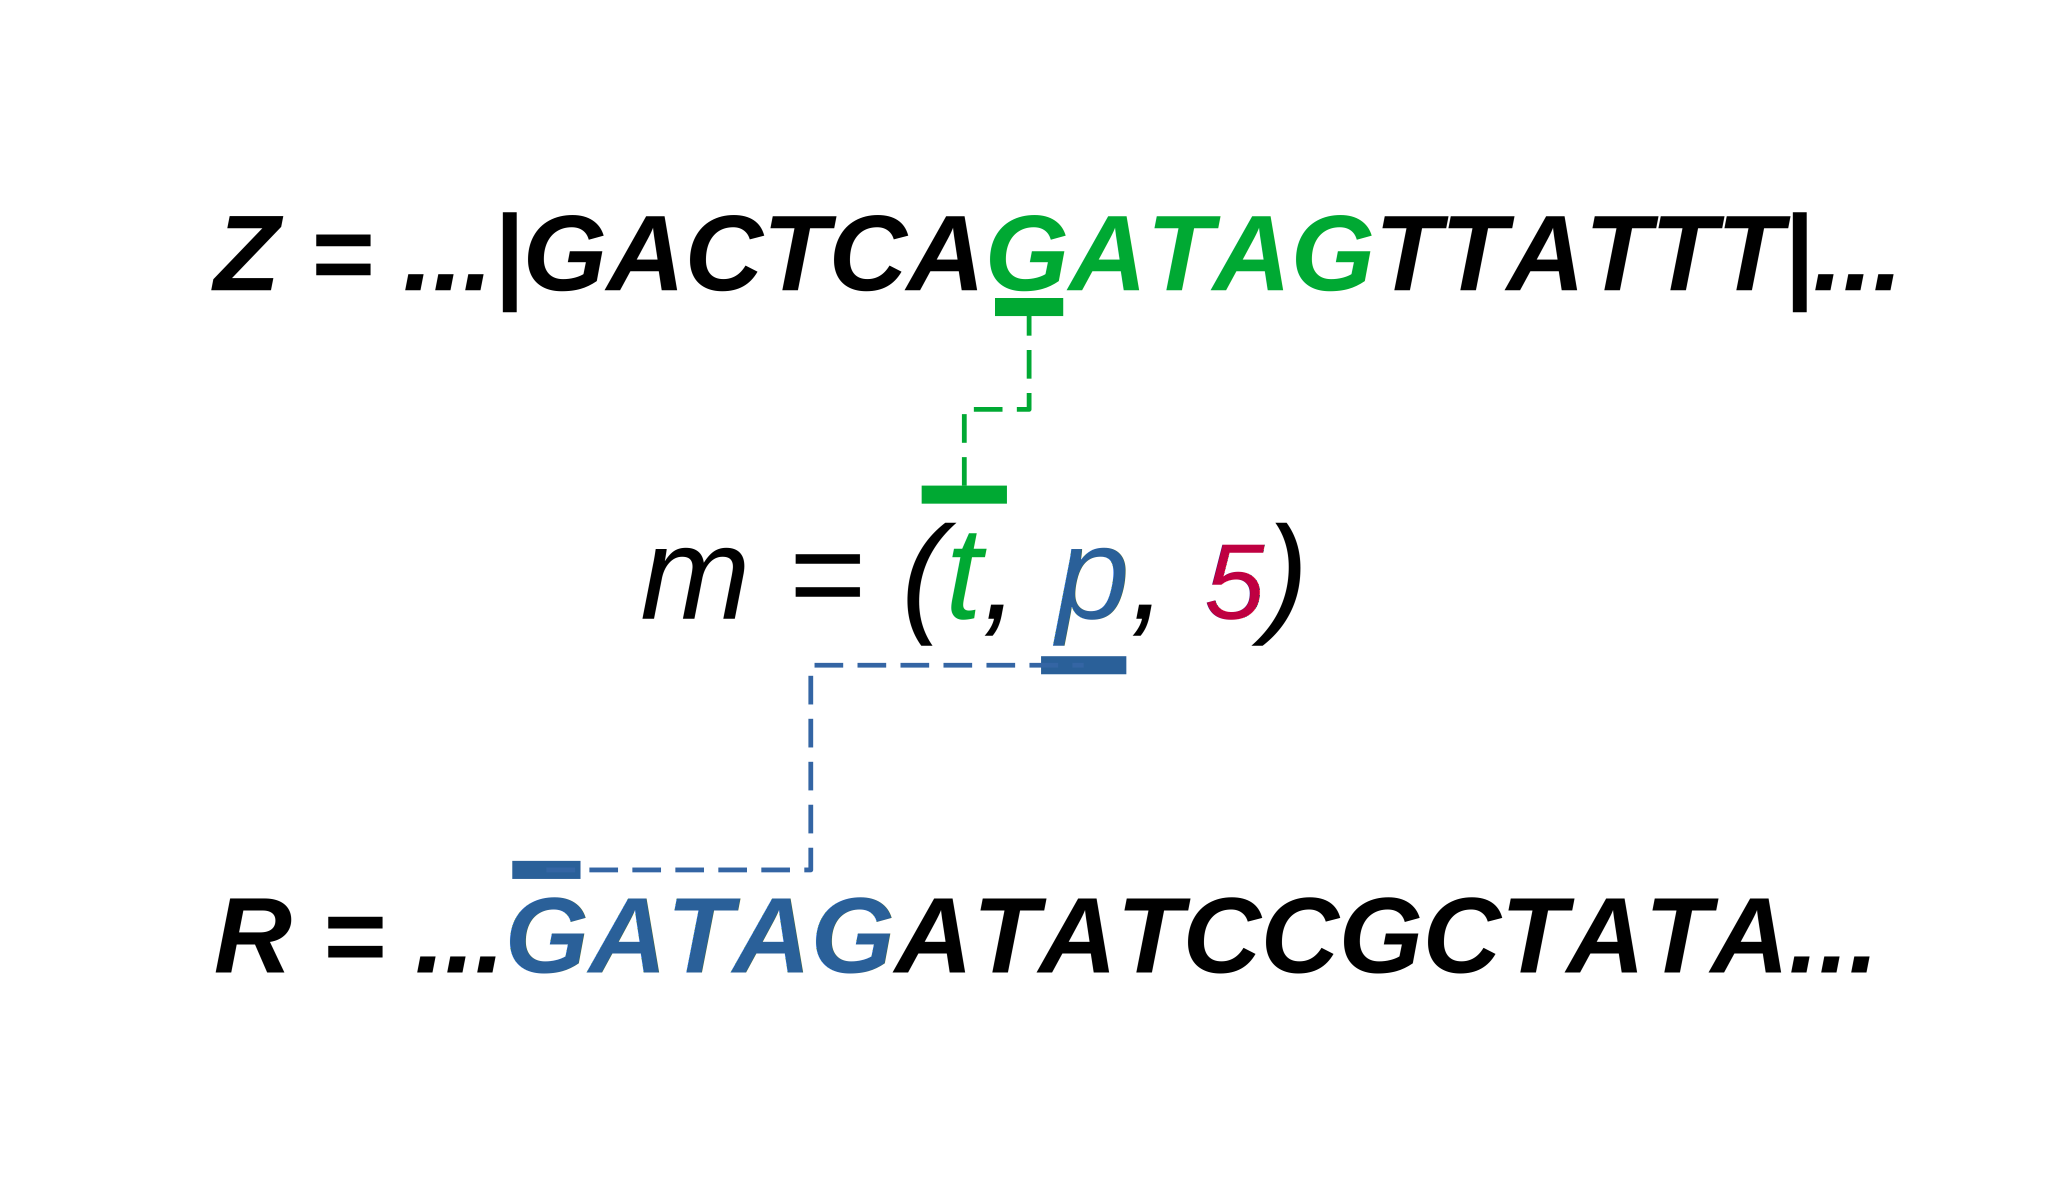
\includegraphics[scale = 0.65]{img/mem.jpg}

  \end{columns}
  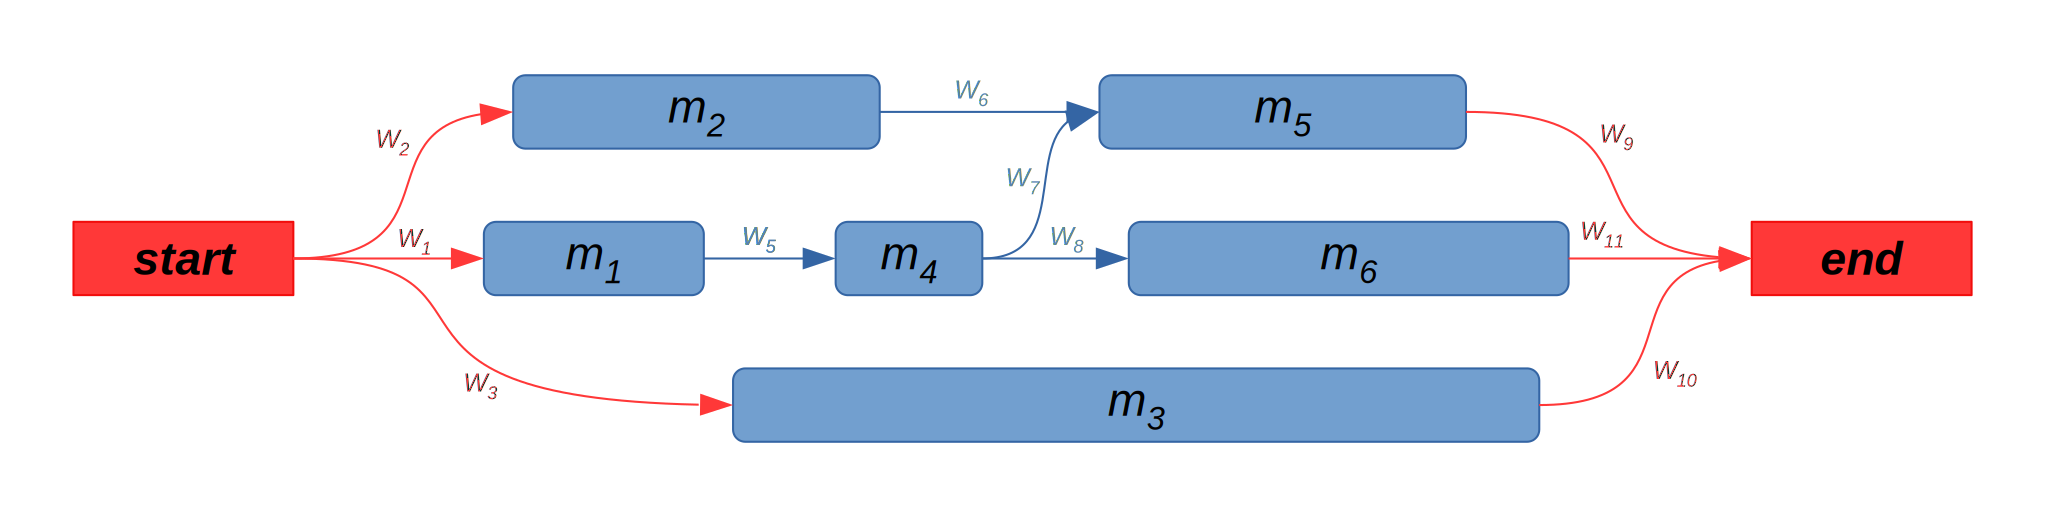
\includegraphics[scale = 0.315]{img/memg.png}

\end{tframe}


\begin{tframe}{Innovazioni: riconoscimento degli introni}
  % \begin{itemize}
  %   \item riconoscimento, per ogni trascritto, delle sequenze complementari a
  %   quelle degli esoni e aggiunta all'insieme dei possibili introni eventuali
  %   esoni presenti solo in alcuni trascritti
  %   \item costruzione della linearizzazione degli introni e della mappa che
  %   associa gli \textit{ID} di due esoni consecutivi alla lista degli
  %   \textit{ID} degli introni in essi contenuti, trascurando il trascritto di
  %   provenienza 
  % \end{itemize}
  \begin{itemize}
    \item riconoscimento degli introni a partire dall'annotazione
    \item costruzione della linearizzazione degli introni
    \item costruzione della mappa degli introni
  \end{itemize}
  % \begin{center}
  %   \includegraphics[scale = 0.31]{img/intron2.png}
  % \end{center}
  \begin{center}
     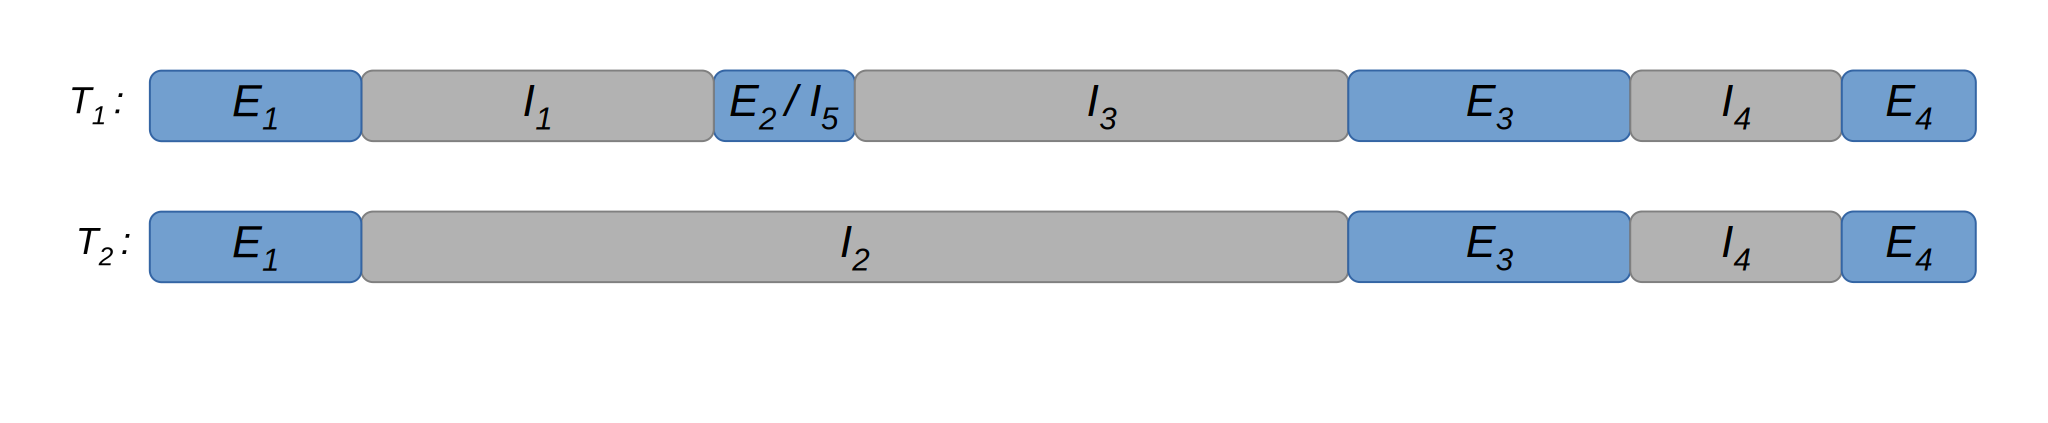
\includegraphics[scale = 0.39]{img/intron.jpg}
   \end{center}
  \begin{block}<1->{Mappa degli introni associata ai due trascritti}
    \begin{itemize}
      \item $(E_1,\,E_2) = [I_1]$
      \item $(E_1,\,E_3) = [I_1,\,I_2,\,I_3,\,I_5]$
      \item $(E_2,\,E_3) = [I_3]$
      \item $(E_3,\,E_4) = [I_4]$
    \end{itemize}
  \end{block}
\end{tframe}

\begin{tframe}{Innovazioni: estensione del MEMs graph}
  \begin{center}
    $\tikzmarkin<1->{c}\tikzmarkin<1>{d}
    m=(t,\,p,\,l,\,\{0,\,1\})\,
    \tikzmarkend{d}\tikzmarkend{c}$
  \end{center}
  \begin{center}
    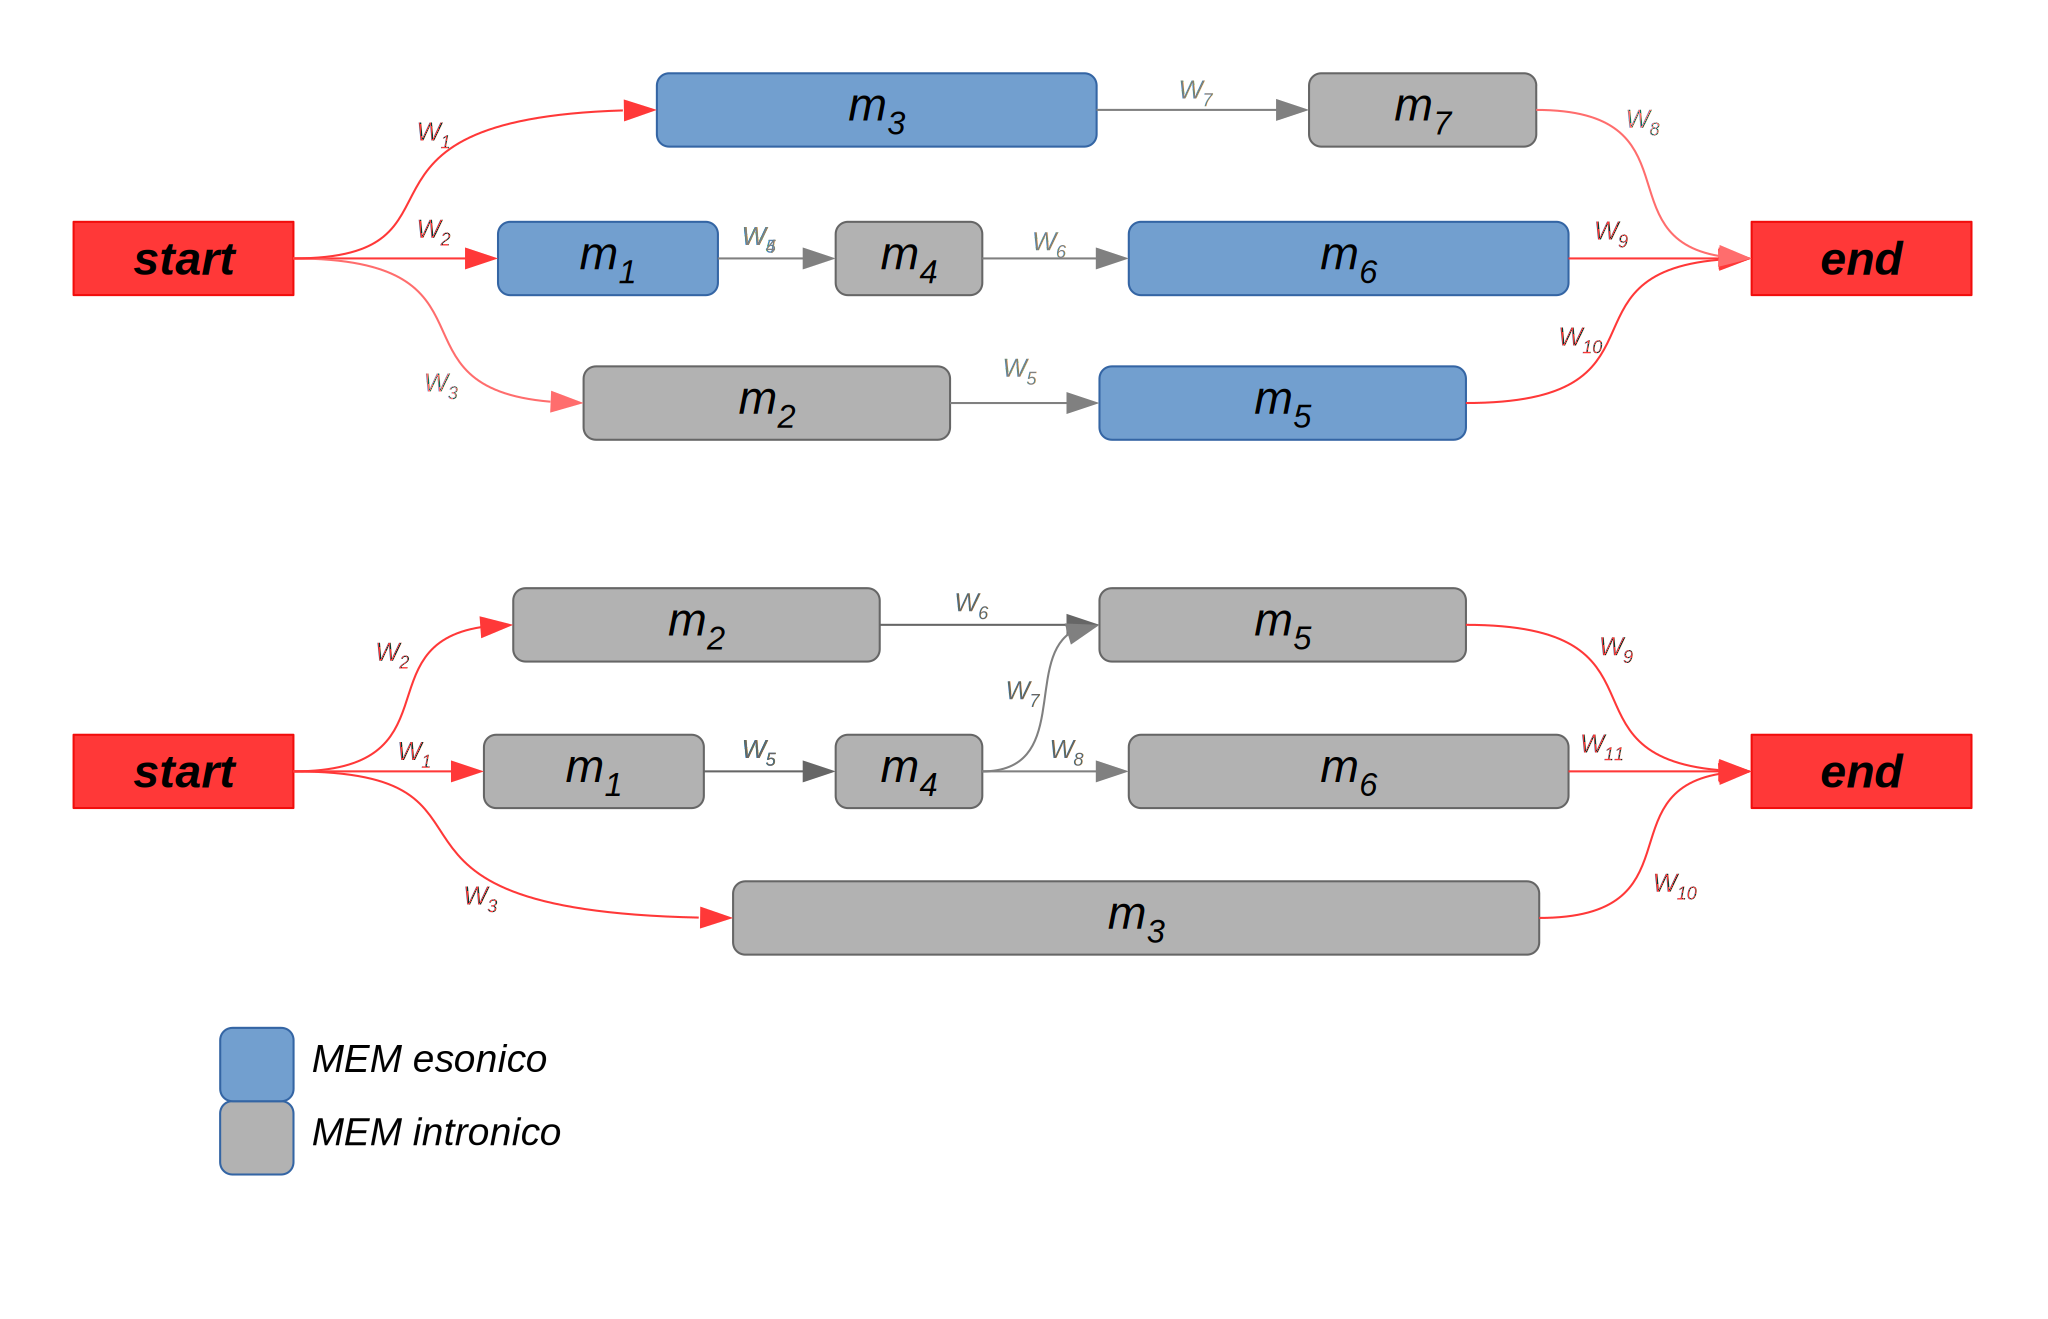
\includegraphics[scale = 0.27]{img/memi.png}
  \end{center}
\end{tframe}

% \begin{tframe}{Analisi dei risultati, visualizzazione con IGV}
%  \textit{Studio iniziale su una piccola annotazione:}
%  \vspace{2.5mm}

%  \includegraphics[width=1\columnwidth, height=2.8cm]{img/igvorig.jpg}
%  \includegraphics[width=1\columnwidth, height=2.8cm]{img/igvi.jpg}   

% \end{tframe}

% \begin{tframe}{Analisi dei risultati, sperimentazione con Snakemake}
%   \begin{columns}
%     \column{0.37\textwidth}
%     \begin{itemize}
%       \item download del genoma e dell'annotazione
%       \vspace{2mm}
%       \item manipolazione dell'annotazione
%       \vspace{2mm}
%       \item calcolo dei \textbf{MEMs}
%       \vspace{2mm}
%       \item produzione dei risultati
%     \end{itemize}
%     \column{0.57\textwidth}
%     % \includegraphics[scale = 0.27]{img/graph.jpg}
%     \includegraphics[scale = 0.27]{img/graph.jpg}
%   \end{columns}

% \end{tframe}
% \begin{tframe}{Analisi dei risultati, sperimentazione con Snakemake}
%   \begin{columns}
%     \column{0.37\textwidth}
%     \begin{itemize}
%       \item download del genoma e dell'annotazione
%       \vspace{2mm}
%       \item manipolazione dell'annotazione
%       \vspace{2mm}
%       \item calcolo dei \textbf{MEMs}
%       \vspace{2mm}
%       \item produzione dei risultati
%     \end{itemize}
%     \column{0.57\textwidth}
%     % \includegraphics[scale = 0.27]{img/graph.jpg}
%     \includegraphics[scale = 0.17]{img/graph.jpg}
%   \end{columns}
%     \begin{center}
%     \resizebox{\textwidth}{!}{%
%     \begin{tabular}{c|c|c|c|c|c|c|c|c}
%       \hline
%       \cellcolor[gray]{0.8} \fontsize{9pt}{9pt}\selectfont cromosoma &
%       \cellcolor[gray]{0.8}\fontsize{9pt}{9pt}\selectfont error rate&
%       \cellcolor[gray]{0.8}\fontsize{9pt}{9pt}\selectfont tipo &
%        \cellcolor[gray]{0.8}\fontsize{9pt}{9pt}\selectfont match &
%       \cellcolor[gray]{0.8}\fontsize{9pt}{9pt}\selectfont$\leq$10\% &
%       \cellcolor[gray]{0.8}\fontsize{9pt}{9pt}\selectfont $>$10\%
%       & \cellcolor[gray]{0.8}\fontsize{9pt}{9pt}\selectfont mismatch &
%        \cellcolor[gray]{0.8}\fontsize{9pt}{9pt}\selectfont tempo (s) &
%       \cellcolor[gray]{0.8}\fontsize{9pt}{9pt}\selectfont memoria (Mb)\\
      
%       \hline

%       \multirow{2}{*}{\small{9}}  &  \multirow{2}{*}{\small{1\%}} & \small{intron} & 24747 & 194 & 23 & 36 & 9.6 & 59.1\\
%                                                                 & & \small{noIntron} & 22993 & 64 & 6 & 1937 & 4.6 & 57.2\\
%       \hline
      
%       \multirow{2}{*}{\small{9}}  &  \multirow{2}{*}{\small{10\%}} & \small{intron} & 24748 & 193 & 23 & 36 & 10.0 & 49.7\\
%                                                                 & & \small{noIntron} & 22991 & 64 & 6 & 1939 & 4.6s & 49.5\\
%       \hline
%     \end{tabular}}
%   \end{center}
% \end{tframe}
\begin{tframe}{Innovazioni: sperimentazione e analisi dei risultati}
  \begin{columns}
    \column{0.55\textwidth}
    \begin{itemize}
      \item download del genoma e dell'annotazione
      \item manipolazione dell'annotazione
      \item simulazione dell'RNA-Seq sample\\
      \small{(25000 reads lunghe 100)}
      \item calcolo dei \textbf{MEMs}
      \item produzione e analisi dei risultati
    \end{itemize}
    \column{0.35\textwidth}
    \begin{itemize}
      \item automatizzazione con Snakemake
      \item semplice modifica dei parametri
      \item parallelismo
    \end{itemize}
  \end{columns}

    \begin{center}
    \resizebox{\textwidth}{!}{%
    \begin{tabular}{c|c|c|c|c|c|c|c|c}
      \hline
      \cellcolor[gray]{0.8} \fontsize{9pt}{9pt}\selectfont cromosoma &
      \cellcolor[gray]{0.8}\fontsize{9pt}{9pt}\selectfont error rate&
      \cellcolor[gray]{0.8}\fontsize{9pt}{9pt}\selectfont tipo &
       \cellcolor[gray]{0.8}\fontsize{9pt}{9pt}\selectfont match &
      \cellcolor[gray]{0.8}\fontsize{9pt}{9pt}\selectfont$\leq$10\% &
      \cellcolor[gray]{0.8}\fontsize{9pt}{9pt}\selectfont $>$10\%
      & \cellcolor[gray]{0.8}\fontsize{9pt}{9pt}\selectfont mismatch &
       \cellcolor[gray]{0.8}\fontsize{9pt}{9pt}\selectfont tempo (s) &
      \cellcolor[gray]{0.8}\fontsize{9pt}{9pt}\selectfont memoria (Mb)\\
      
      \hline

      \multirow{2}{*}{\small{9}}  &  \multirow{2}{*}{\small{1\%}} & \small{intron} & 24747 & 194 & 23 & 36 & 9.6 & 59.1\\
                                                                & & \small{noIntron} & 22993 & 64 & 6 & 1937 & 4.6 & 57.2\\
      \hline
      \multirow{2}{*}{\small{9}}  &  \multirow{2}{*}{\small{2\%}} & \small{intron} & 24748 & 194 & 23 & 35 & 9.6 & 59.2\\
                                                                & & \small{noIntron} & 22993 & 64 & 6 & 1937 & 4.6 & 57.9\\
      \hline
      \multirow{2}{*}{\small{9}}  &  \multirow{2}{*}{\small{10\%}} & \small{intron} & 24748 & 193 & 23 & 36 & 10.0 & 49.7\\
                                                                & & \small{noIntron} & 22991 & 64 & 6 & 1939 & 4.6 & 49.5\\
      \hline
    \end{tabular}}
  \end{center}
\end{tframe}

% \begin{tframe}{Analisi dei risultati}
%    \includegraphics[width=1\columnwidth, height=2.8cm]{img/igvi.jpg}   

%     \begin{center}
%     \resizebox{\textwidth}{!}{%
%     \begin{tabular}{c|c|c|c|c|c|c|c|c}
%       \hline
%       \cellcolor[gray]{0.8} \fontsize{9pt}{9pt}\selectfont cromosoma &
%       \cellcolor[gray]{0.8}\fontsize{9pt}{9pt}\selectfont error rate&
%       \cellcolor[gray]{0.8}\fontsize{9pt}{9pt}\selectfont tipo &
%        \cellcolor[gray]{0.8}\fontsize{9pt}{9pt}\selectfont match &
%       \cellcolor[gray]{0.8}\fontsize{9pt}{9pt}\selectfont$\leq$10\% &
%       \cellcolor[gray]{0.8}\fontsize{9pt}{9pt}\selectfont $>$10\%
%       & \cellcolor[gray]{0.8}\fontsize{9pt}{9pt}\selectfont mismatch &
%        \cellcolor[gray]{0.8}\fontsize{9pt}{9pt}\selectfont tempo (s) &
%       \cellcolor[gray]{0.8}\fontsize{9pt}{9pt}\selectfont memoria (Mb)\\
      
%       \hline

%       \multirow{2}{*}{\small{9}}  &  \multirow{2}{*}{\small{1\%}} & \small{intron} & 24747 & 194 & 23 & 36 & 9.6 & 59.1\\
%                                                                 & & \small{noIntron} & 22993 & 64 & 6 & 1937 & 4.6 & 57.2\\
%       \hline
%       \multirow{2}{*}{\small{9}}  &  \multirow{2}{*}{\small{2\%}} & \small{intron} & 24748 & 194 & 23 & 35 & 9.6 & 59.2\\
%                                                                 & & \small{noIntron} & 22993 & 64 & 6 & 1937 & 4.6s & 57.9\\
%       \hline
%       \multirow{2}{*}{\small{9}}  &  \multirow{2}{*}{\small{10\%}} & \small{intron} & 24748 & 193 & 23 & 36 & 10.0 & 49.7\\
%                                                                 & & \small{noIntron} & 22991 & 64 & 6 & 1939 & 4.6s & 49.5\\
%       \hline
%     \end{tabular}}
%   \end{center}
% \end{tframe}



% \begin{tframe}{Analisi dei risultati, esiti della sperimentazione}
%   \textit{Sperimentazione con \textbf{RNA-Seq sample} da 25000 reads lunghe
%     100:} 
%   % \vspace{2cm}
%   \begin{center}
%     \resizebox{\textwidth}{!}{%
%     \begin{tabular}{c|c|c|c|c|c|c|c|c}
%       \hline
%       \cellcolor[gray]{0.8} \fontsize{9pt}{9pt}\selectfont cromosoma &
%       \cellcolor[gray]{0.8}\fontsize{9pt}{9pt}\selectfont error rate&
%       \cellcolor[gray]{0.8}\fontsize{9pt}{9pt}\selectfont tipo &
%        \cellcolor[gray]{0.8}\fontsize{9pt}{9pt}\selectfont match &
%       \cellcolor[gray]{0.8}\fontsize{9pt}{9pt}\selectfont$\leq$10\% &
%       \cellcolor[gray]{0.8}\fontsize{9pt}{9pt}\selectfont $>$10\%
%       & \cellcolor[gray]{0.8}\fontsize{9pt}{9pt}\selectfont mismatch &
%        \cellcolor[gray]{0.8}\fontsize{9pt}{9pt}\selectfont tempo (s) &
%       \cellcolor[gray]{0.8}\fontsize{9pt}{9pt}\selectfont memoria (Mb)\\
      
%       \hline
%       \multirow{2}{*}{\small{1}}  &  \multirow{2}{*}{\small{1\%}}& \small{intron} & 24727 & 212 & 29 &
%                                                                                                       32
%                                                                       & 14.9 & 148.7\\
%                                                                 & &\small{noIntron} & 23026 & 75 & 7 & 1892 & 4.4 & 139.1\\
%       \hline
%       \multirow{2}{*}{\small{9}}  &  \multirow{2}{*}{\small{1\%}} & \small{intron} & 24747 & 194 & 23 & 36 & 9.6 & 59.1\\
%                                                                 & & \small{noIntron} & 22993 & 64 & 6 & 1937 & 4.6 & 57.2\\
%       \hline
%       \multirow{2}{*}{\small{9}}  &  \multirow{2}{*}{\small{2\%}} & \small{intron} & 24748 & 194 & 23 & 35 & 9.6 & 59.2\\
%                                                                 & & \small{noIntron} & 22993 & 64 & 6 & 1937 & 4.6s & 57.9\\
%       \hline
%       \multirow{2}{*}{\small{9}}  &  \multirow{2}{*}{\small{10\%}} & \small{intron} & 24748 & 193 & 23 & 36 & 10.0 & 49.7\\
%                                                                 & & \small{noIntron} & 22991 & 64 & 6 & 1939 & 4.6s & 49.5\\
%       \hline
%       \multirow{2}{*}{\small{21}}  &  \multirow{2}{*}{\small{1\%}} & \small{intron} & 24732 & 220 & 26  & 22 & 8.1 & 30.6 \\
%                                                                 & & \small{noIntron} & 22750 & 85 & 9 & 2156 & 3.9s & 29.7\\
%       \hline
%     \end{tabular}}
%   \end{center}
% \end{tframe}ù


\begin{tframe}{Conclusioni e prospettive future}
  \begin{block}<1->{Considerazioni sui risultati}
    \begin{adv}
      \item buona qualità dei risultati
    \end{adv}
    \begin{disadv}
      \item performances (tempi medi di esecuzione) non ottimali
    \end{disadv}
  \end{block}
  \vspace{5mm}
  
   \begin{block}<2->{Prospettive future}
     \begin{itemize}
       \item ottimizzazione dello studio degli introni
       \item perfezionamento del \textbf{MEMs graph}
       \item parallelizzazione dello studio delle reads
     \end{itemize}
  \end{block}
\end{tframe}
\title{Grazie per l'attenzione}
\ateneo{Ringraziamenti}
\titlepageframe

\end{document}
% LocalWords:  splicing graph MEMs linearizzazione vector Matches
